\documentclass{standalone}
  \usepackage{tikz}
  \usetikzlibrary{arrows.meta, automata, bending, positioning, shapes.misc}
  \tikzstyle{automaton}=[shorten >=1pt, >={Stealth[bend,round]}, initial text=]
  \tikzstyle{accepting}=[accepting by arrow]

\begin{document}
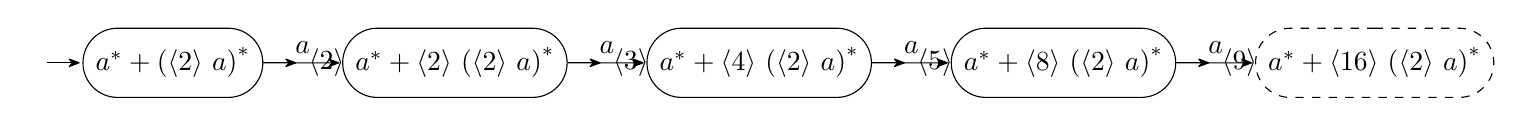
\begin{tikzpicture}[automaton, auto]
  \node[state,initial,accepting,accepting text=$\left\langle 2\right\rangle$,rounded rectangle] (0) {${a}^{*} + \left( \left\langle 2 \right\rangle \,a\right)^{*}$};
  \node[state,accepting,accepting text=$\left\langle 3\right\rangle$,rounded rectangle] (1) [right=of 0] {${a}^{*} +  \left\langle 2 \right\rangle \,\left( \left\langle 2 \right\rangle \,a\right)^{*}$};
  \node[state,accepting,accepting text=$\left\langle 5\right\rangle$,rounded rectangle] (2) [right=of 1] {${a}^{*} +  \left\langle 4 \right\rangle \,\left( \left\langle 2 \right\rangle \,a\right)^{*}$};
  \node[state,accepting,accepting text=$\left\langle 9\right\rangle$,rounded rectangle] (3) [right=of 2] {${a}^{*} +  \left\langle 8 \right\rangle \,\left( \left\langle 2 \right\rangle \,a\right)^{*}$};
  \node[state,dashed,rounded rectangle] (4) [right=of 3] {${a}^{*} +  \left\langle 16 \right\rangle \,\left( \left\langle 2 \right\rangle \,a\right)^{*}$};
  \path[->] (0) edge node {$a$} (1);
  \path[->] (1) edge node {$a$} (2);
  \path[->] (2) edge node {$a$} (3);
  \path[->] (3) edge node {$a$} (4);
\end{tikzpicture}
\end{document}
